\section{Finite interactions can reverse a local damping decision}
\label{sec:decision}
The following result addresses a narrower, executed decision than a maximum
replacement claim. A site may retune its PLL after SG replacement to preserve
the real part of one mode in the full network. Combining two such individually
compensated actions need not preserve that modal margin. ``Damping-only'' here
means the modal decay rate $-\Re\lambda$, not the damping ratio or a diagonal
entry of the physical impedance. The two meanings are not interchangeable.

\subsection{Exact local actions and the interaction left after them}
Let $F_0(s)$ denote the affine full descriptor at a fixed equilibrium and fixed
physical delays. Partition the intervention representation into site blocks:
\begin{equation}
 F(s,d)=F_0(s)+\mathcal U\Theta(d)\mathcal V(s),\quad
 H=\Theta(d)\mathcal V(s)F_0(s)^{-1}\mathcal U .
\end{equation}
Each site has four channels but three independent physical actions: the two
replacement channels share the same $\delta\rho_i$. Let $F_i$ change only
site $i$, keeping the entire physical network. On a common contour $\Gamma$,
write
\begin{equation}
 B_i=I+H_{ii},\qquad K_{ij}=B_i^{-1}H_{ij}\ (i\ne j),\qquad K_{ii}=0.
\end{equation}
Assume $F_0$, each $F_i$ and the joint $F$ are holomorphic regular descriptors
inside $\Gamma$, have no boundary roots, and enclose the same number $m>0$ of
physical roots. Require the displayed inverses on the boundary. These
conditions are checked, not inferred from a small singular-value residual.
If $z_0,z_i,z$ are the respective mean enclosed roots, define
\begin{equation}
 z_N=z_0+\sum_i(z_i-z_0),\qquad \mathcal I=z-z_N .
 \label{eq:singleton-counterfactual}
\end{equation}
$z_N$ is an exact-singleton additive counterfactual. It already contains the
physical network in every singleton calculation; it is not a published
decentralized stability certificate or an independently realizable system.

\begin{proposition}[Finite pair interaction without a weak-coupling assumption]
For exactly two active sites $i,j$, set $P=K_{ij}K_{ji}$. For any $c\in\mathbb C$,
\begin{align}
 \frac{\det F\det F_0}{\det F_i\det F_j}
 &=\det(I-P),\label{eq:pair-determinant}\\
 \boxed{\mathcal I=-\frac{1}{2\pi\ii m}\oint_\Gamma(s-c)
 \operatorname{tr}\big[(I-P)^{-1}P_s\big]\,ds.}\label{eq:pair-rational}
\end{align}
No condition $\rho(P)<1$ is needed in this identity.
\end{proposition}
\begin{proof}
The determinant lemma gives $\det F/\det F_0=\det(I+H)$.
Factoring $\diag(B_i,B_j)$ gives
$\det(I+H)=\det B_i\det B_j\det\left[\begin{smallmatrix}I&K_{ij}\\K_{ji}&I\end{smallmatrix}\right]$.
The last determinant is $\det(I-P)$, while
$\det F_i/\det F_0=\det B_i$. Differentiate the scalar determinant ratio
and apply the argument-principle first moment. Equal counts make the
constant $c$ vanish. This proof uses logarithmic derivatives, not a
globally selected matrix logarithm. $K$ may be meromorphic in the interior.
\end{proof}
\status{EXACT\_IDENTITY}
This is an application of established determinant and contour identities.
Its role is to separate finite, physically realizable singleton effects
from their joint correction, including parameter-dependent mode changes.

For implementation,
\begin{equation}
 (K_{ij})_s=B_i^{-1}\big[(H_{ij})_s-(H_{ii})_sK_{ij}\big],\qquad
 P_s=(K_{ij})_sK_{ji}+K_{ij}(K_{ji})_s.
\end{equation}
The two-step interaction and its exact rational remainder are
\begin{align}
 C_2&=\frac{1}{2\pi\ii m}\oint_\Gamma\operatorname{tr}P\,ds,\\
 \mathcal I-C_2&=-\frac{1}{2\pi\ii m}\oint_\Gamma(s-c)
 \operatorname{tr}\big[(I-P)^{-1}P P_s\big]\,ds.\label{eq:rational-remainder}
\end{align}
The second identity follows by splitting $(I-P)^{-1}=I+(I-P)^{-1}P$
and integrating $\oint(s-c)\operatorname{tr}P_s=-\oint\operatorname{tr}P$.
An absolute-integrand bound or a direct signed interval integral encloses
the remainder. When the two actions scale to zero, its local order is
four. In contrast, the positive walk-series bound requires
$\rho(|K_{ij}||K_{ji}|)<1$; it must be abandoned when that condition fails.
$C_2$ resums within-site effects and is not generally a degree-two polynomial
in the finite actions. These loops connect intervention ports through the
whole network; they are not identified with physical transmission cycles.

\subsection{A finite exclusion and a compensation rule}
Suppose $m=1$ and the required real-part margin is $-\sigma$.
Enclosures $\Re z_N\le n_+$ and $\Re(z_N+\mathcal I)\ge a_-$ prove an
incorrectly permissive singleton prediction when
\begin{equation}
 n_++\sigma<0,\qquad a_-+\sigma>0.\label{eq:finite-decision}
\end{equation}
For $m>1$, a positive mean margin still proves that at least one root violates
the requirement; a negative mean does not prove every root passes.
This excludes the specified joint design, not every allowed local controller.

To correct the decision, keep the replacement and prescribed $K_p$ fixed.
Let physical singleton maps exist with
$\Re z_i(r_i)=\alpha_0-r_i$, valid gains, and fixed positive weights
$r_i=w_i t$, $\sum_iw_i=1$. Write $I(t)=\Re\mathcal I(t)$ and
$b=-\alpha_0-\sigma>0$. The exact joint margin is
\begin{equation}
 \boxed{g(t)=-b-t+I(t),\qquad t^*=I(t^*)-b.}\label{eq:budget-fixedpoint}
\end{equation}
The variable $t$ is an allocated modal-decay budget in $\mathrm{s}^{-1}$;
it is neither gain effort nor replacement MW.

\begin{theorem}[Conditional finite compensation budget]
Suppose the singleton maps, gain bounds and common root counts hold for
$0\le t\le Q$. If $I(0)>b$, $|I'(t)|\le\kappa<1$ throughout that interval,
and $Q\ge[I(0)-b]/(1-\kappa)$, there is a unique crossing and
\begin{equation}
 \frac{I(0)-b}{1+\kappa}\le t^*\le
 \frac{I(0)-b}{1-\kappa}.
\end{equation}
The iteration $t_{k+1}=\max\{0,I(t_k)-b\}$ converges from $[0,Q]$.
Every $t\in[t^*,Q]$ passes this enclosed-root margin condition.
\end{theorem}
\begin{proof}
The clipped map is $\kappa$-Lipschitz, maps $[0,Q]$ into itself and has
a unique fixed point. It is positive since its value at zero is positive.
The bound follows from $|I(t^*)-I(0)|\le\kappa t^*$.
Finally, $g'(t)=-1+I'(t)<0$. This is a specialization of contraction and
monotonicity arguments, not a new general convergence theorem.
\end{proof}
\status{PROVED\_REDUCED\_MODEL}
Here ``reduced'' concerns the scalar budget and enclosed-root constraint;
the spectral functions can be evaluated on the exact full DDE. A sampled
derivative bound is insufficient to invoke the uniform theorem.

\paragraph{What can be composed exactly.}
If every additive descriptor intervention satisfies
$\delta F_i(\lambda_*)v_*=0$ for the \emph{same} nonzero vector $v_*$ and
$F_0(\lambda_*)v_*=0$, then their sum preserves that eigenpair.
Preserving only a real part, or even preserving the same eigenvalue with
different eigenvectors, does not imply this condition. The full-network
all-PLL construction in Appendix~\ref{sec:closure} supplies a way to impose
a common pattern; it is a separate design choice, not proof of optimality.

\subsection{Executed IEEE--39 decision and its falsifiers}
The numerical values, figures and tables below are generated from
\path{experiments/interaction_decision_20261004/}.
The original grids produced no valid false acceptance and five modal false
rejections; failed tracking comparisons were retained. A second campaign
combined individually complex-pole-preserving replacements and found no
margin violations in its 230 cases. Its largest adverse shift was below
$3\times10^{-5}\,\mathrm{s}^{-1}$, too small to substantiate the intended
material failure. Both negative findings are retained.

The adaptive third campaign increased each selected site's $\rho$ by 0.01,
prescribed a $2\%$ increase in $K_p$, and solved its $K_i$ and modal frequency
while preserving the real part. The selected sites are 30 and 37. Selection
was by the saved smallest-step rule; it was not an independent validation
sample. The all-case table retains 405 designs, of which 88 were resolved
and two violated the selected margin. The remaining 317 were unresolved
or failed the declared frequency guard and are not labeled harmless.

\begin{center}\small
\begin{tabular}{lrr}\toprule
Design & $\Re\lambda$ ($\mathrm{s}^{-1}$) & Additional GFL MW\\\midrule
Anchor & $-0.06570893$ & 0.00\\
Bus30 alone & $-0.06570893$ & 2.50\\
Bus37 alone & $-0.06570893$ & 5.40\\
Joint actions & $-0.04139961$ & 7.90\\
Complex-pole rule & $-0.06570803$ & 7.90\\
Interaction correction & $-0.06000000$ & 7.90\\
\bottomrule\end{tabular}
\end{center}
The displayed root centers have certified coordinate radii $10^{-7}$ before display rounding.
\status{NUMERICALLY\_VALIDATED} With rigorous ball enclosures of the exported model, the real interaction lies in $0.024309321\pm4.01\times10^{-7}\,\mathrm{s}^{-1}$, including display rounding.
The joint design violates the required margin while each singleton passes its enclosed-root condition. It remains asymptotically decaying at this pole; margin violation is not a claim of instability.
\begin{figure}[ht]\centering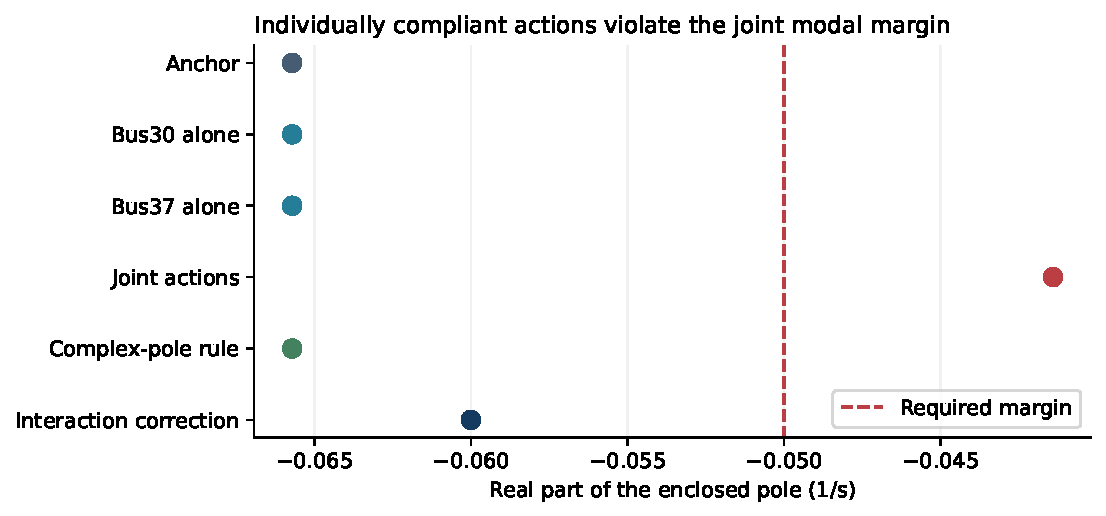
\includegraphics[width=.94\linewidth]{experiments/interaction_decision_20261004/FIG_01_CERTIFIED_DECISION.pdf}\caption{The finite modal decision reversal and two alternative corrections. Error bars are smaller than the markers.}\end{figure}
The equal-budget fixed-point correction targets $-0.06\,\mathrm{s}^{-1}$ and converged in 11 updates to $t=0.01700492\,\mathrm{s}^{-1}$. It changes $K_i$ at buses 30 and 37 to 272.416969 and 288.703323; their prescribed $K_p=28.839821$ is unchanged. The largest sampled absolute interaction slope was 0.3850; this is not a verified uniform contraction constant.
\begin{figure}[ht]\centering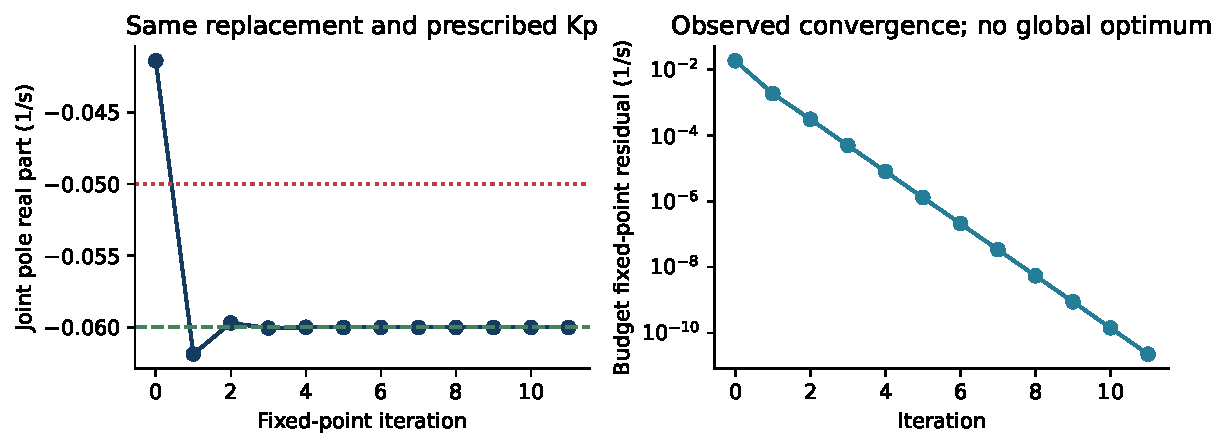
\includegraphics[width=.97\linewidth]{experiments/interaction_decision_20261004/FIG_02_COMPENSATION_RULE.pdf}\caption{Executed scalar compensation rule. Its endpoint root is certified, while convergence beyond this run remains conditional.}\end{figure}
The corrected design contains 4735.316 MW GFL (87.64622\%) and 667.445 MW retained SG. These are prescribed feasible-design coordinates, not maxima.
Along the separately declared independent tuning policy, the first numerical margin crossing has certified endpoint signs at 6.38445 and 6.38604 additional MW. This is not a global replacement bound; interval-wide monotonicity is not certified.
Independent Julia linearization reproduces the exported model. The floating-point complete-region DDE contour test returns anchor: 0 violating roots, single30: 0 violating roots, single37: 0 violating roots, joint: 2 violating roots, complex pair: 0 violating roots, corrected: 0 violating roots. These counts are numerical; the interval certificates above have their explicitly smaller scope.
The frozen nonlinear DDE campaign passes 5/5 events, with maximum frequency excursion 0.465874 Hz, maximum windowed RoCoF 0.219060 Hz/s and minimum retained-SG actuator slack 0.008918. Frequency and RoCoF use 0.5 s windows. No converter current-limiter safety is asserted.

\paragraph{Certified scope.}
Complex-ball arithmetic at 160-bit precision encloses the source CSV values,
gains and delays as their exact binary64 values. The algebraic elimination
is enclosed. A balanced open-loop resolvent series encloses its numerical
evaluation without approximating the exponential delay. Positive-oriented
argument-principle contours prove one simple physical root in each small
square. Four additional common-contour counts prove that the baseline,
singletons and joint design refer to a common one-root region. This connects
their finite difference to Eq.~\eqref{eq:pair-rational}.
The interval enclosure certifies the endpoint correction itself; the
two-step approximation is only numerical because its walk-series gate failed.

\paragraph{Comparison and novelty boundary.}
The ordinary quadratic prediction also detects this violation, although less
accurately. Thus the example does not establish that only the resummed method
can make the correct decision. It establishes a finite, certified failure
of additive singleton prediction and an executed correction rule.
Classical multivariable interaction analysis already uses normalized
off-diagonal return maps \cite{grosdidier}. A recent IBR block-dominance
certificate also accounts for inter-device interaction and a prescribed
decay rate \cite{chenbdd}; it is not the additive surrogate falsified here.
No claim of first publication, globally optimal replacement, GSP compression,
necessity of communication, or a new physical-line-cycle law follows.
